\documentclass{beamer}

\usepackage{graphicx}
\usepackage{bibentry}
\graphicspath{ {./images/} }

\title{Analyse von Pflanzenwachstum auf Basis von 3D-Punktwolken}

\author{Jakob Görner} 
\institute[Computer Vision] 
{HSNR - Master Arbeit - Vortrag \\ % Your institution for the title page
\medskip
\textit{jakob.goerner@stud.hn.de} % Your email address

}

\usefonttheme{default}
%\usetheme{lucid}
\begin{document}
\frame {
	\titlepage
}
\frame {
	\frametitle{Inhalt} 
	\tableofcontents
}
\section{Ziele}
\frame {
	\sffamily
	\frametitle{Ziele} 
	\begin{itemize}
		\item Analyse von Pflanzen mittels 3D-Punktwolken
		\begin{itemize}
			\item Größe
			\item Anzahl Blätter
			\item Biomasse
			\item ...
		\end{itemize}
		\item Generierung von Punktwolken auf Basis von Bildern
		\item Kernprobleme
		\begin{itemize}
			\item Entfernung des Hintergrundes
			\item Segmentierung der Pflanze
			\item Skalierung der Punktwolken ist unbekannt.
		\end{itemize}
		\item REST-Interface zum einspielen von Datensätzen und ansteuern der Funktionalitäten.
		\item Datenübertragung zum Server sollte gering gehalten werden.
	\end{itemize}
}

\section{Generierung von Punktwolken}
\frame{
	\frametitle{Generierung von Punktwolken} 
	\begin{itemize}
		\item Einsatz von spezieller Hardware sollte nicht nötig sein.
		\begin{itemize}
			\item Hohe Anschaffungskosten
			\item Bedienung ist nicht trivial
			\item Daher Structure from Motion (SfM)
			\item SfM ermöglicht die Generierung von Punktwolken aus einer Menge an Bildern.
		\end{itemize}
		\item Da es viele bestehende Lösungen für SfM existieren, wird auf eine existierende Implementationen zurück gegriffen.
		\item Voraussetzungen an die Implementation
		\begin{itemize}
			\item Möglichst wenig Bilder sollten reichen für gute Ergebnisse.
			\item Performance der Implementation sollte möglichst gut sein.
			\item Keine Information über Kamera Position und Ausrichtung.
			\item Gegebenenfalls keine Information über die Reihenfolge der Bilder.
		\end{itemize}
\end{itemize}
}

\frame{
	\frametitle{Generierung von Punktwolken} 
	\begin{itemize}
	\item Evaluation mehrerer Implementationen
	\begin{itemize}
		\item Open Drone Map \cite{ODM}
		\item Colmap \cite{schoenberger2016sfm}
		\item AliceVision (Meshroom) \cite{Moulon2012}
		\item OpenMVG \cite{moulon2016openmvg} 
		\item OpenCV SFM Pipeline
	\end{itemize}
	\item Open Drone Map(ODM) und Colmap liefern gute Ergebnisse.
	\item Colmap liefert die besser Auflösung.
	\item ODM ist wesentlich performanter als Colmap (schnellere Berechnung bei weniger Ressourcen-Verbrauch).
	\item ODM ermittelt eine besser Abdeckung der Oberfläche.
	\item ODM liefert zusätzlich eine Schätzung der Normalen für jeden Punkt.
\end{itemize}
}

\frame{
	\frametitle{Generierung von Punktwolken} 
	\begin{figure}
		\centering
		\begin{minipage}{0.475\textwidth}
			\centering
			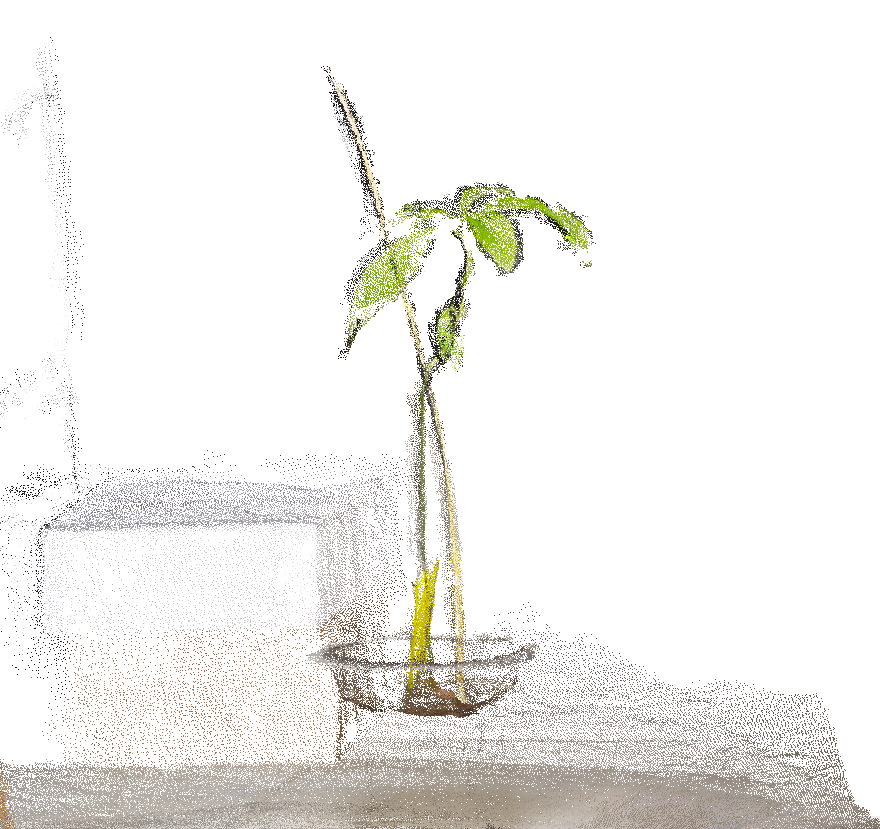
\includegraphics[width=1.0\textwidth]{./Images/PointCloudGeneration_odm.png}
			\caption{ODM}
			\label{fig:odm}
		\end{minipage}\hfill
		\begin{minipage}{0.475\textwidth}
			\centering
			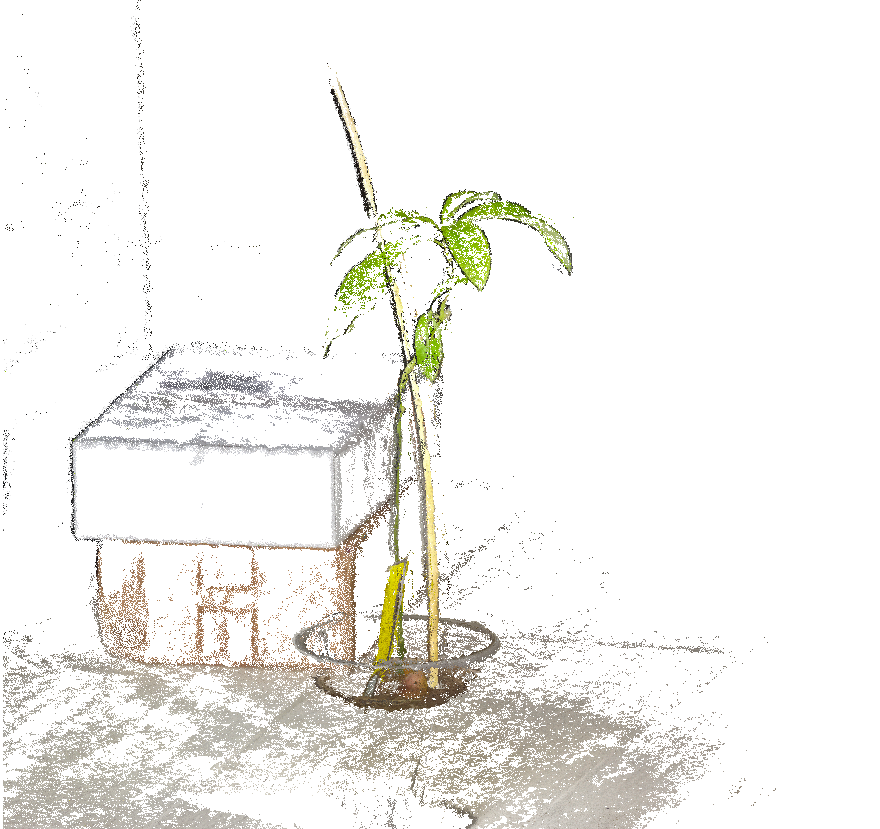
\includegraphics[width=1.0\textwidth]{./Images/PointCloudGeneration_colmap.png}
			\caption{Colmap}
			\label{fig:colmap}
		\end{minipage}
	\end{figure}
}
\frame{
	\frametitle{Generierung von Punktwolken} 
	\begin{figure}
		\centering
		\begin{minipage}{0.3\textwidth}
			\centering
			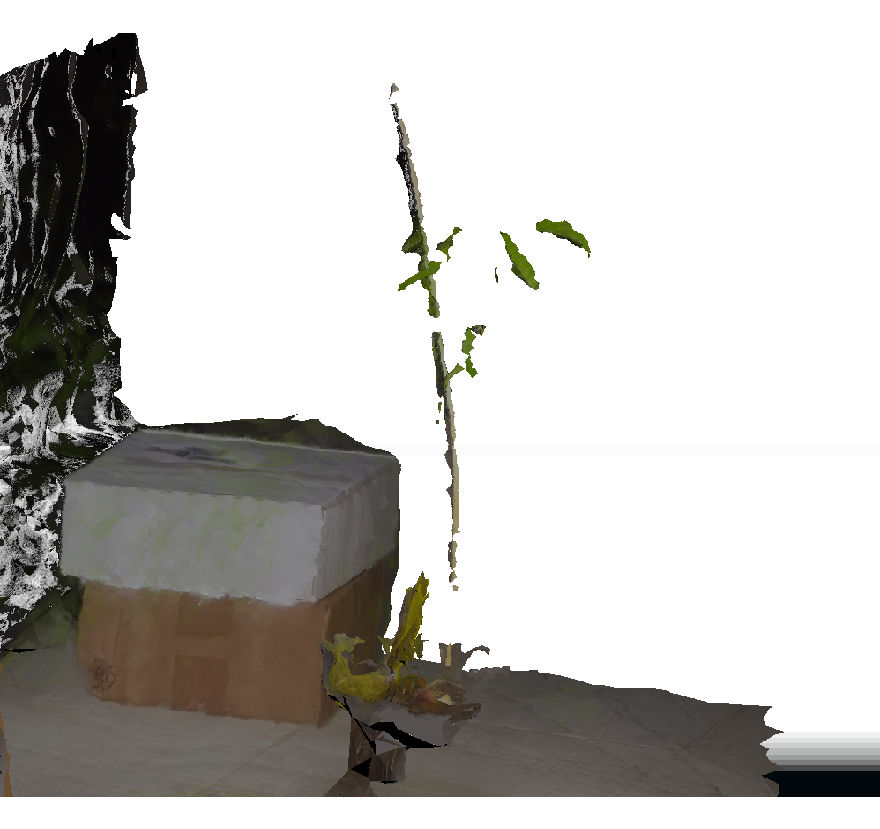
\includegraphics[width=1.0\textwidth]{./Images/PointCloudGeneration_meshroom.png}
			\caption{Meshroom}
			\label{fig:meshroom}
		\end{minipage}\hfill
		\begin{minipage}{0.3\textwidth}
			\centering
			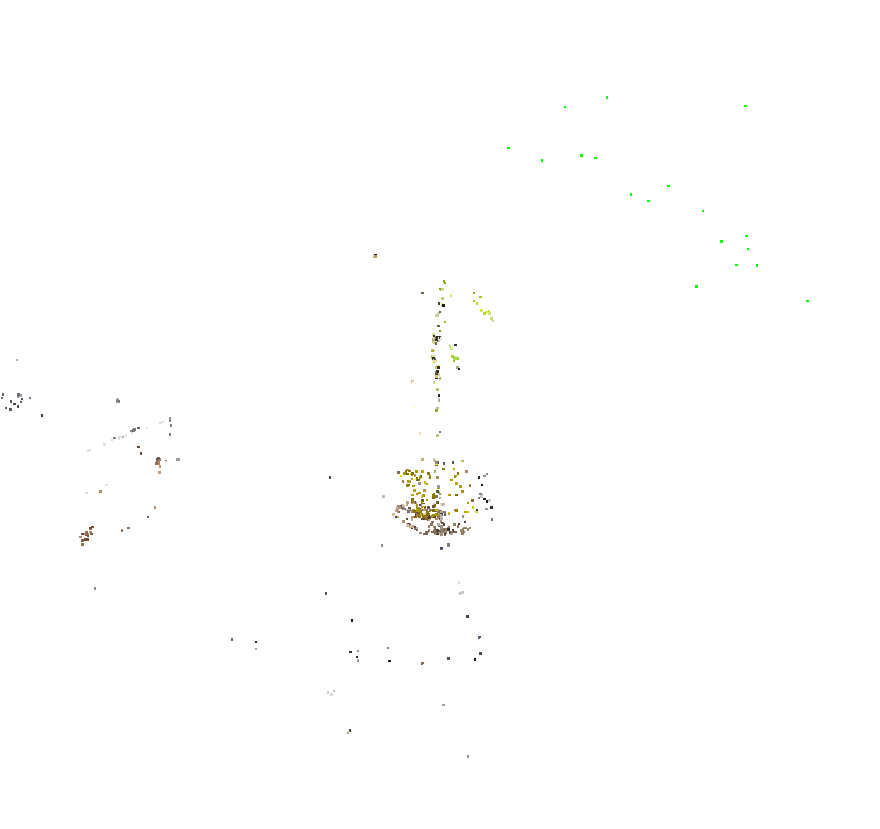
\includegraphics[width=1.0\textwidth]{./Images/PointCloudGeneration_openmvg.png}
			\caption{OpenMVG}
			\label{fig:openmvg}
		\end{minipage}\hfill
		\begin{minipage}{0.3\textwidth}
			\centering
			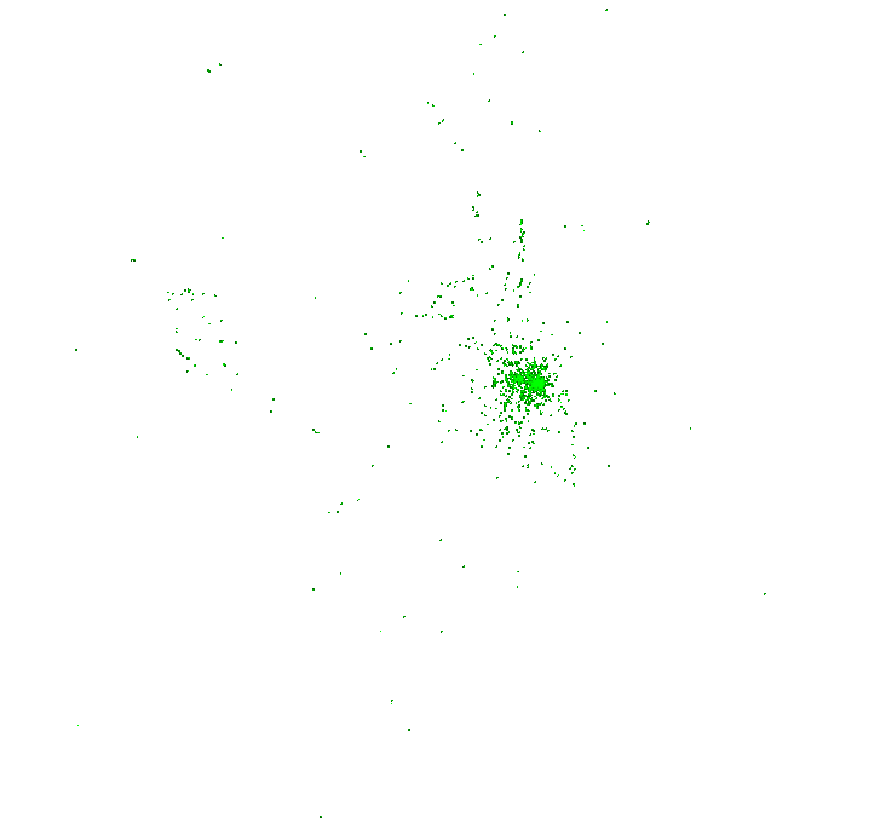
\includegraphics[width=1.0\textwidth]{./Images/PointCloudGeneration_opencv.png}
			\caption{OpenCV}
			\label{fig:opencv}
		\end{minipage}
	\end{figure}
}

\section{Segmentierung}
\frame{
	\frametitle{Segmentierung - Pflanze} 
	\begin{itemize}
		\item Ansatz 1: Entscheidung auf Basis der Krümmung eines Punktes
		\item Je höher die Krümmung eines Punktes ist desto wahrscheinlicher gehört dieser zu einem Stiel.
		\item Problem: Es muss eine gute Parametrisierung für alle Pflanzen-Arten gefunden werden.
		\item Problem: Blätter haben teilweise ähnlich Krümmung wie Stiele.
		\item Nachteil: Entfernung des Hintergrundes bleibt offen.
		\item Nachteil: Es liegt lediglich ein binärer Classifier vor. Es können nur die Stiele von dem Rest der Pflanze differenziert werden.
		\item Nachteil: Es müssen Normalen bekannt sein.
	\end{itemize}
}
\frame{
	\frametitle{Segmentierung - Pflanze} 
	\begin{figure}
		\centering
		\begin{minipage}{0.475\textwidth}
			\centering
			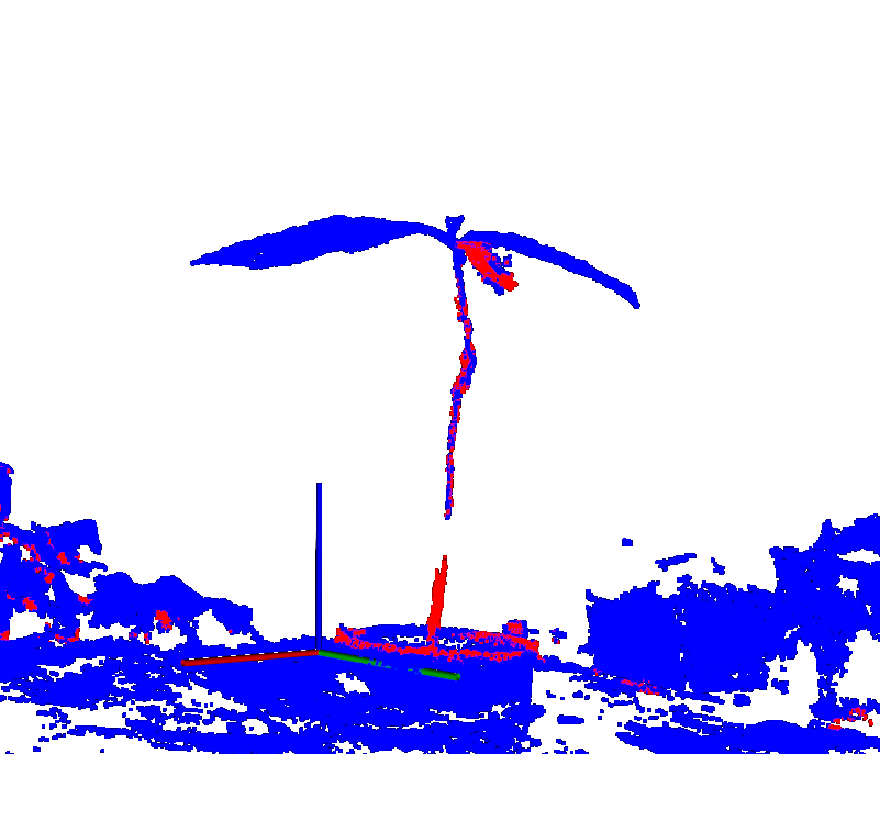
\includegraphics[width=1.0\textwidth]{./Images/HandcraftedClassifierAvocado.png}
			\caption{Avocado Ansatz 1}
			\label{fig:classifier:1}
		\end{minipage}\hfill
		\begin{minipage}{0.475\textwidth}
			\centering
			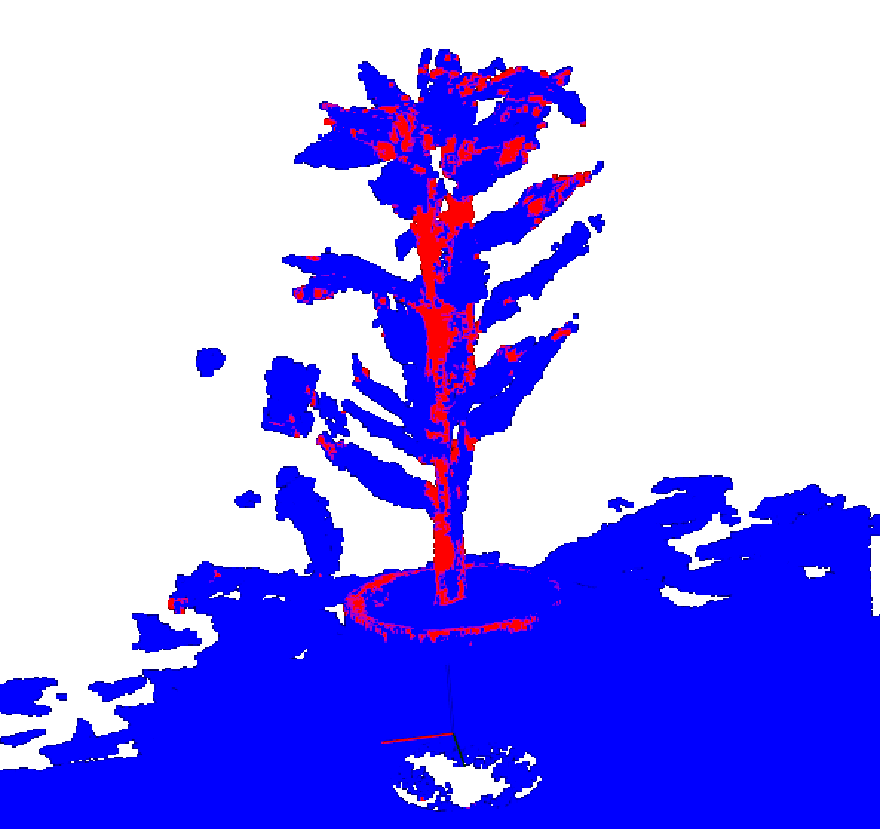
\includegraphics[width=1.0\textwidth]{./Images/HandcraftedClassifierPlant2.png}
			\caption{Zimmerpflanze Ansatz 1}
			\label{fig:classifier:2}
		\end{minipage}
	\end{figure}
}
\frame{
	\frametitle{Segmentierung - Pflanze} 
	\begin{itemize}
		\item Ansatz 2: Nutzung von Neuronalen Netzen (PointNet++)
		\item Erstellen eines Trainings-Datensatz aus 144 individuelle Punktwolken, mit bis zu 20 Subsamples je Punktwolke.
		\item Nutzung des Datensatzes in verschiedenen Trainings-Szenarien.
		\item Vorteil: Neben Blättern und Stielen können weitere Klassen segmentiert werden. 
		\item Nachteil: Erstellen der Trainings-Daten sehr Zeit aufwendig + Daten müssen verfügbar sein.
	\end{itemize}
}
\frame{
	\frametitle{Segmentierung - Pflanze} 
	\begin{figure}
		\centering
		\begin{minipage}{0.475\textwidth}
			\centering
			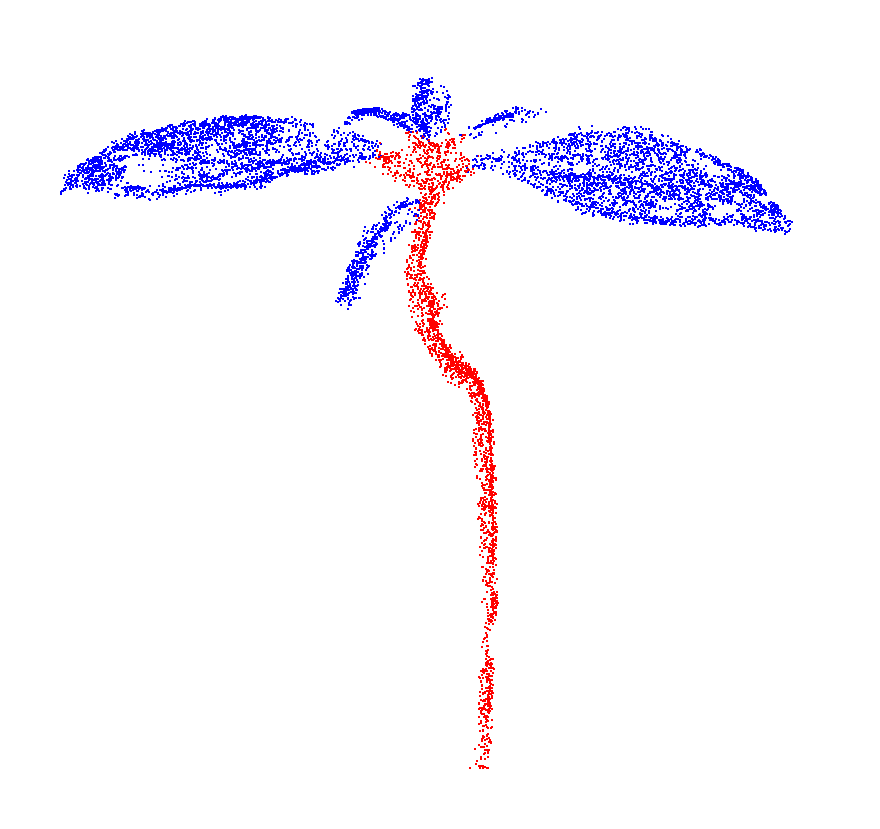
\includegraphics[width=1.0\textwidth]{./Images/Plant_Avocado.png}
			\caption{Avocado Ansatz 2}
			\label{fig:classifier:1}
		\end{minipage}\hfill
		\begin{minipage}{0.475\textwidth}
			\centering
			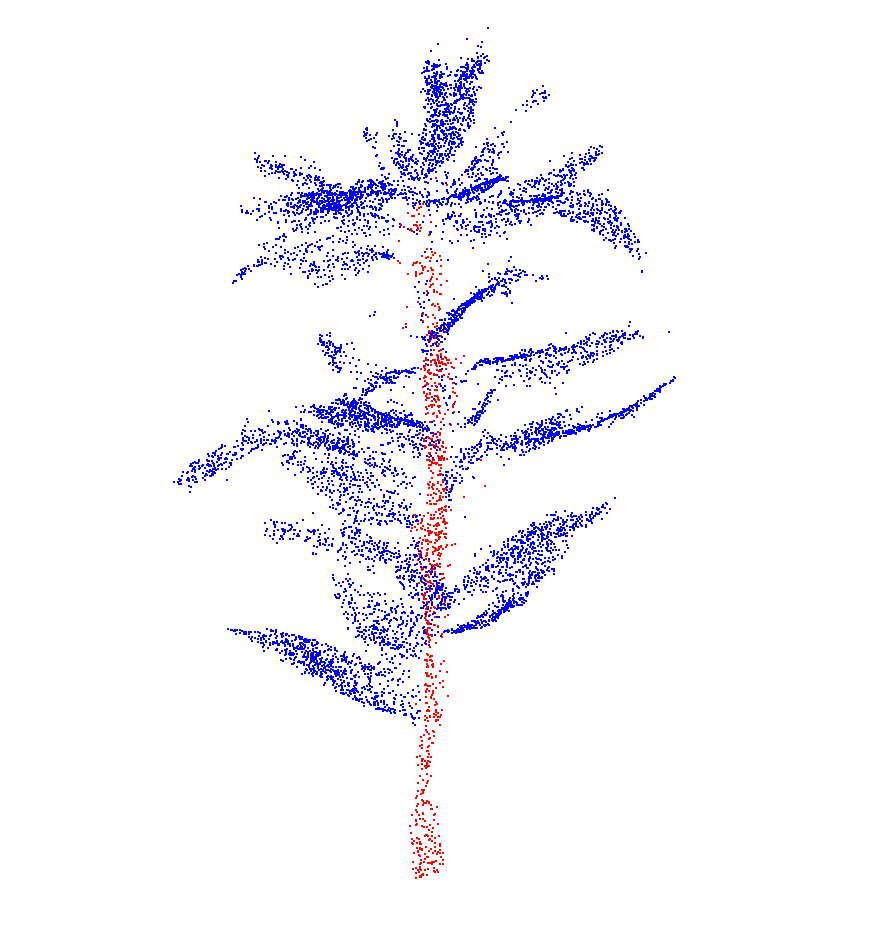
\includegraphics[width=1.0\textwidth]{./Images/Plant_Plant2.png}
			\caption{Zimmerpflanze Ansatz 2}
			\label{fig:classifier:2}
		\end{minipage}
	\end{figure}
}
\frame{
	\frametitle{Segmentierung - Hintergrund} 
	\begin{itemize}
		\item Auch hier wurde PointNet++ verwendet.
		\item Ergebnisse der Hintergrundsegmentierung sind durch den großen Anteil der Hintergrund-Punkte teilweise fehlerhaft.
		\item Pflanzen die ungewollt mit in der Szene enthalten sind, werden mit in die Analyse aufgenommen.
		\item Hier besser eine Szenen-Analyse durchführen und auf Bereichen die als Pflanze erkannt wurde Hintergrund-Segmentierung anwenden um Pflanze freizustellen.
	\end{itemize}
}
\frame{
	\frametitle{Segmentierung - Hintergrund} 
	\begin{figure}
		\centering
		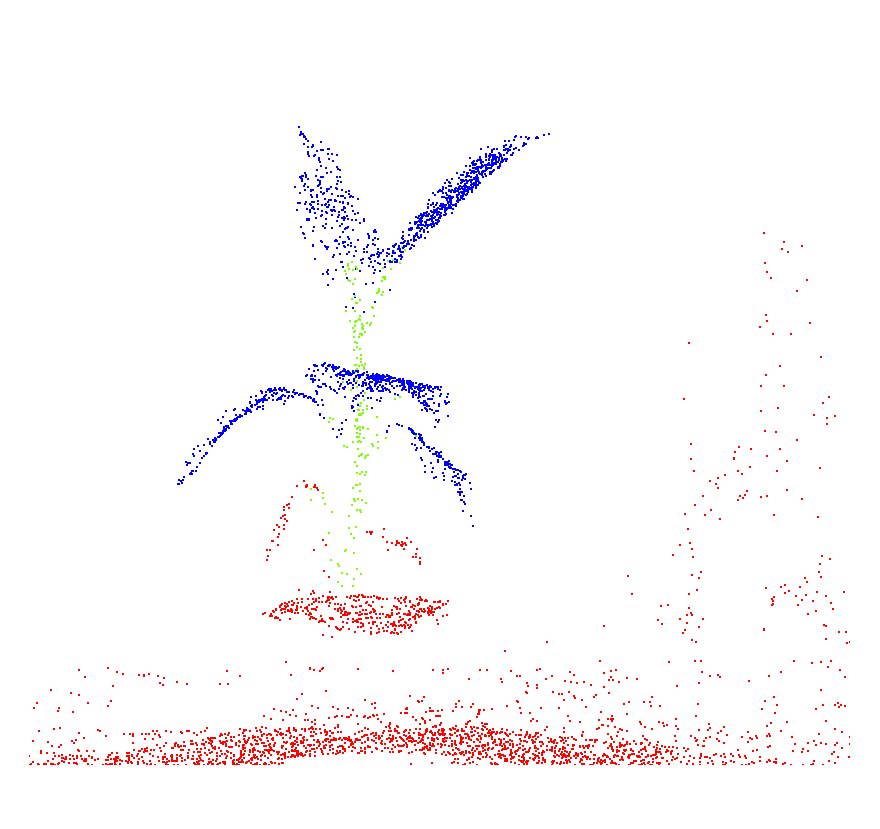
\includegraphics[width=0.65\textwidth]{./Images/BG_Banana.png}
		\caption{Ergebnis Hintergrundsegmentierung}
		\label{fig:background}
	\end{figure}
}
	
\section{Registrierung}
\frame{
	\frametitle{Registrierung} 
	\begin{itemize}
		\item Problem: Da beim Erstellen der Punktwolke mit SfM der Maßstab nicht ermittelt werden kann, liegen verschiedene Punktwolken derselben Szene in unterschiedlichen Maßstäben vor.
		\begin{equation}
			\label{eq:icp}
			\underset{R,t}{\operatorname{argmin}}(\sum_{i=1}^N{\|Rp_{s_i} + t - p_{t_i}\|^2})
		\end{equation}
		\item Lösung: Daher müssen Punktwolken zu unterschiedlichen Zeitpunkten miteinander registriert werden.
		\item Problem: Die meisten Registrierungsverfahren berücksichtigen nicht die Skalierung.
		\item Es wurden mehrere Ansätze untersucht dieses Problem zu lösen.
		\item Grundgedanke: Punktwolken mit einer Hintergrund-Punktwolke registrieren.
	\end{itemize}
}
\frame{
	\frametitle{Registrierung - ICP mit Schätzung der Skalierung} 
	\begin{itemize}
		\item In der Bibliothek Point Cloud Libary (PCL) wird eine Implementation die auch einen Wert für die Skalierung liefert bereit gestellt.
		\item Problem: ICP benötigt gute Initialisierung.
		\item Initialisierung finden:
		\begin{itemize}
			\item Punktwolken an der XY-Ebene ausrichten.
			\item Punktwolken auf die selbe Größe bringen.
			\item Bereich um Zentrum entnehmen.
			\item Punktwolken auf die selbe Größe bringen.
			\item Störung herausfiltern
			\item Registrierung mit SIFT-3D
		\end{itemize}
		\item Nach Schätzung der Skalierung Nachverarbeitung.
		\item Problem: Ansatz funktioniert nur bedingt für einige Punktwolken.
	\end{itemize}
}
\frame{
	\frametitle{Registrierung - DCP anpassen} 
	\begin{itemize}
		\item DCP ist ein Neuronales Netz, welches das Registrierungsproblem löst, aber keine Skalierung liefert.
		\item SVD-Head anpassen und Eingabe mit Einsen erweitern.
		\item Resultat des SVD-Head ist nun eine $4 \times 4$ Matrix.
		\item Annahme das diese Matrix als Transformations-Matrix interpretiert werden kann hat sich nicht bestätigt.
		\item Besser: Berechnung der Skalierung auf Basis der Rotation
	\end{itemize}
}
\frame{
	\frametitle{Registrierung - Iterative Schätzung der Skalierung} 
	\begin{itemize}
		\item Iteratives durchlaufen verschiedener Skalierungen mit anschließender Registrierung.
		\item Für jede Iteration den Abstand der Punktwolke messen und die Iteration wählen, welche den kleinsten Abstand ergab.
		\item Einsatz von verschiedenen Registrierungsverfahren möglich. RPM-Net und ICP haben sich hier als robust erwiesen.
		\item Relativ gute Ergebnisse, aber auch hier kommt es immer wieder zu Ausreißern.
	\end{itemize}
}
\frame{
	\frametitle{Registrierung - Iterative Schätzung der Skalierung} 
	\begin{figure}
		\centering
		\begin{minipage}{0.3\textwidth}
			\centering
			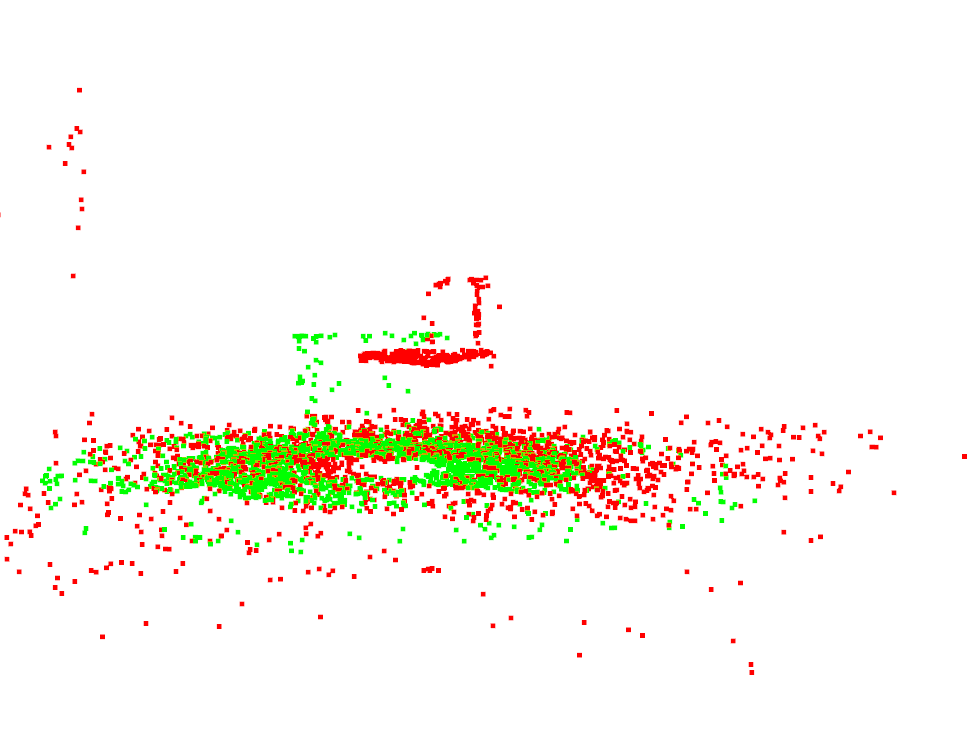
\includegraphics[width=1.0\textwidth]{./Images/RegistrationBananaT1.png}
			\label{fig:meshroom}
		\end{minipage}\hfill
		\begin{minipage}{0.3\textwidth}
			\centering
			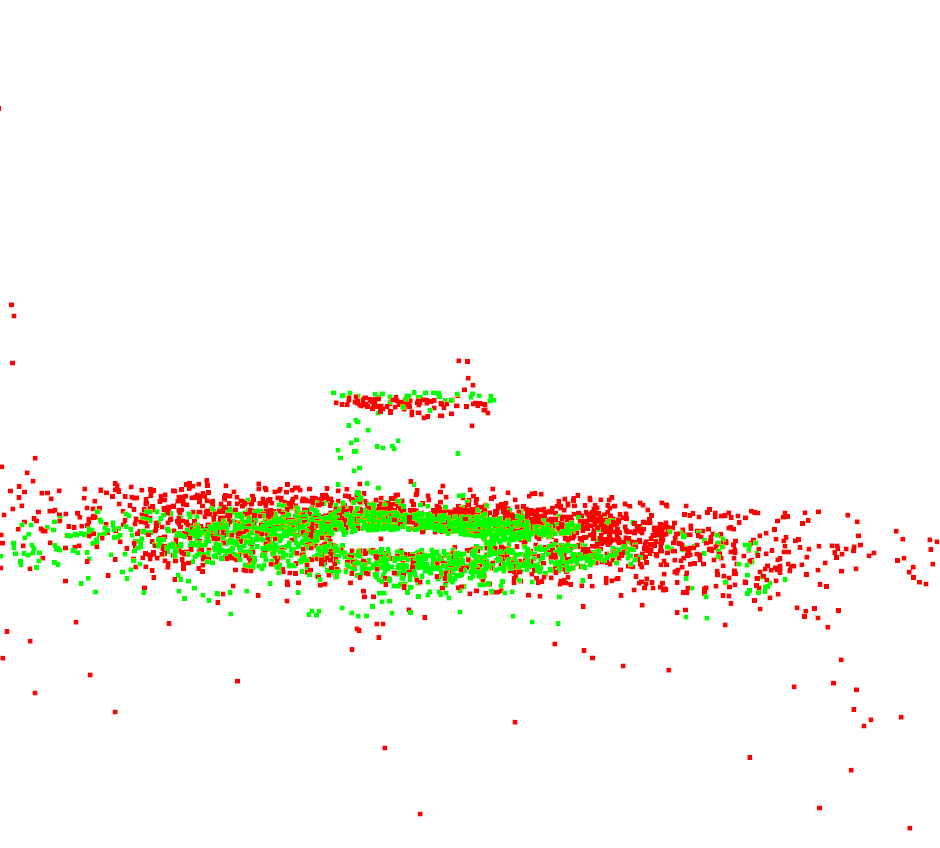
\includegraphics[width=1.0\textwidth]{./Images/RegistrationBananaT2.png}
			\label{fig:openmvg}
		\end{minipage}\hfill
		\begin{minipage}{0.3\textwidth}
			\centering
			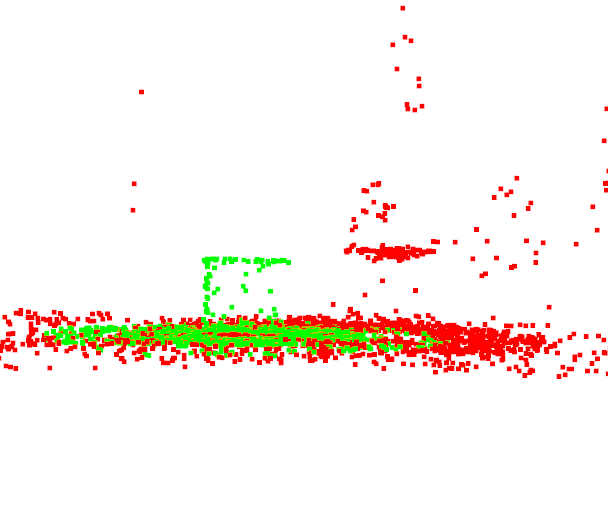
\includegraphics[width=1.0\textwidth]{./Images/RegistrationBananaT3.png}
			\label{fig:opencv}
		\end{minipage}
		\caption{Registrierungsergebnisse für drei Zeitpunkte einer Pflanze}
	\end{figure}
}

\section{Server}
\frame{
	\frametitle{Server} 
	\begin{itemize}
		\item Fünf Schnittstellen um Anwendung zu nutzen.
		\begin{itemize}
			\item POST /detail/\{Messreihe\}/\{Zeitstempel\}
			\item PUT /detail/\{Messreihe\}/\{Zeitstempel\}
			\item GET /detail/\{Messreihe\}/\{Zeitstempel\}
			\item GET /listing/\{Messreihe\}
			\item GET /result/\{Messreihe\}/\{Zeitstempel\}
		\end{itemize}
		\item Bearbeitung einzelner Jobs im Hintergrund.
		\item Zugriffe auf geteilte Ressourcen werden über Mutexe geschützt.
		\begin{itemize}
			\item Job-Queue
			\item Status
			\item Result
		\end{itemize}
	\end{itemize}
}
\frame{
	\frametitle{Server - Pipelines und Jobs} 
	\begin{figure}
		\centering
		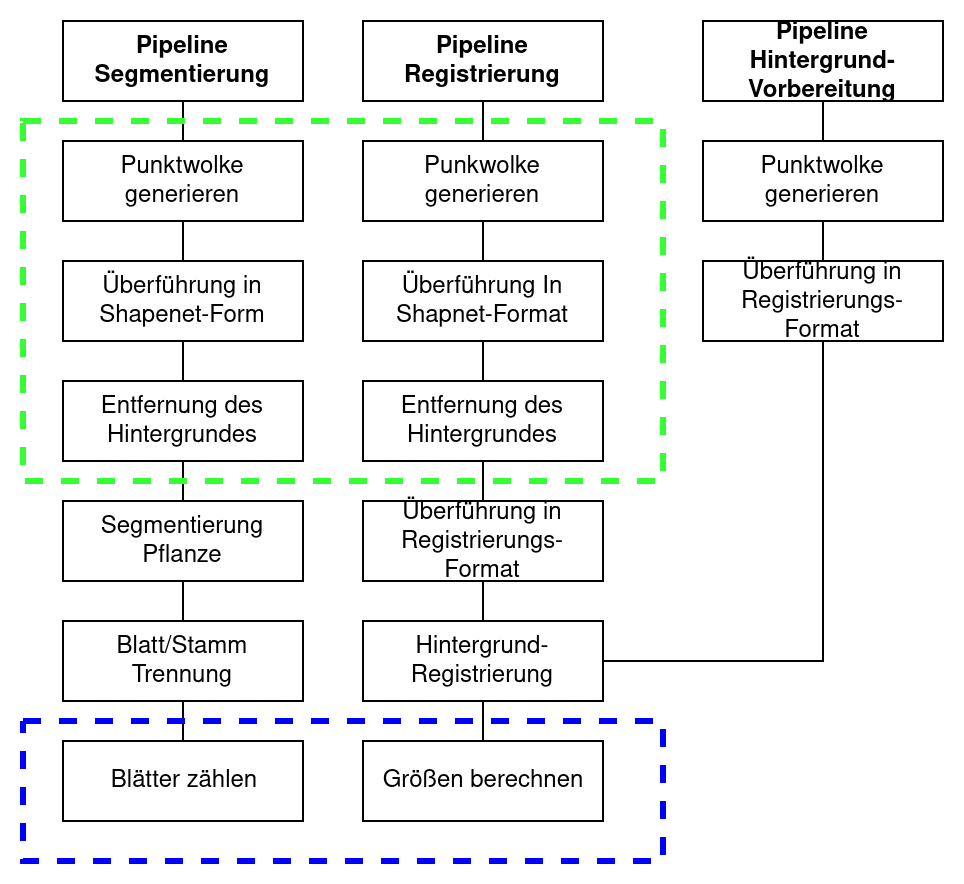
\includegraphics[width=0.65\textwidth]{./Images/Pipelines.png}
		\caption{Übersicht über die einzelnen Pipelines und die darin enthaltenen Jobs.}
		\label{fig:Pipelines}
	\end{figure}
}

\section{Demo}
\frame{
	\frametitle{Demo} 
	\begin{figure}
		\centering
		\begin{minipage}{0.3\textwidth}
			\centering
			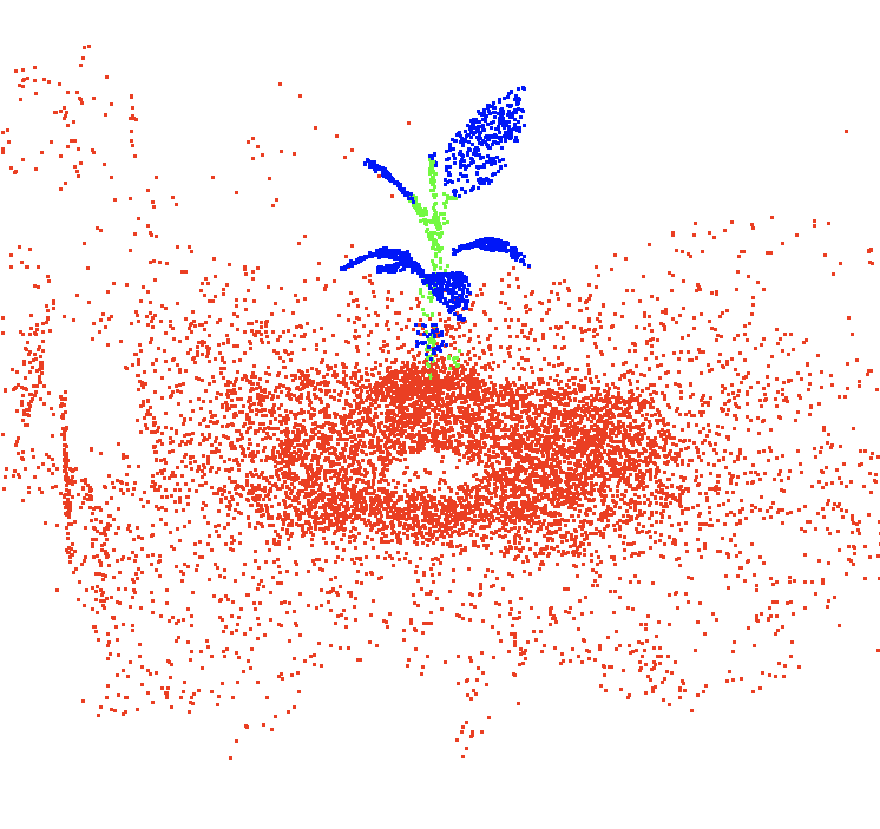
\includegraphics[height=4.5cm,width=4.5cm]{./Images/PipelineBackgroundSegmentationStriped.png}
			\caption{Hintegrund-Segmentierung}
			\label{fig:PiplineBackgroundSegmentation}
		\end{minipage}\hfill
		\begin{minipage}{0.3\textwidth}
			\centering
			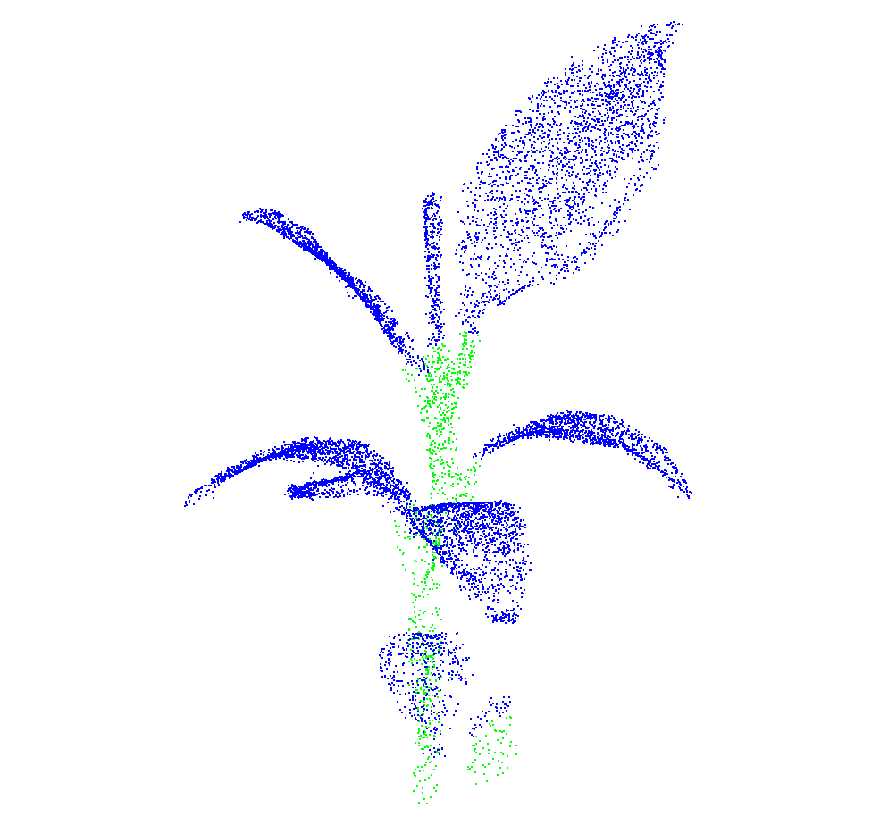
\includegraphics[height=4.5cm,width=4.5cm]{./Images/PipelinePlantSegmentation.png}
			\caption{Planzen-Segmentierung}
			\label{fig:PipelinePlantSegmentation}
		\end{minipage}\hfill
		\begin{minipage}{0.3\textwidth}
			\centering
			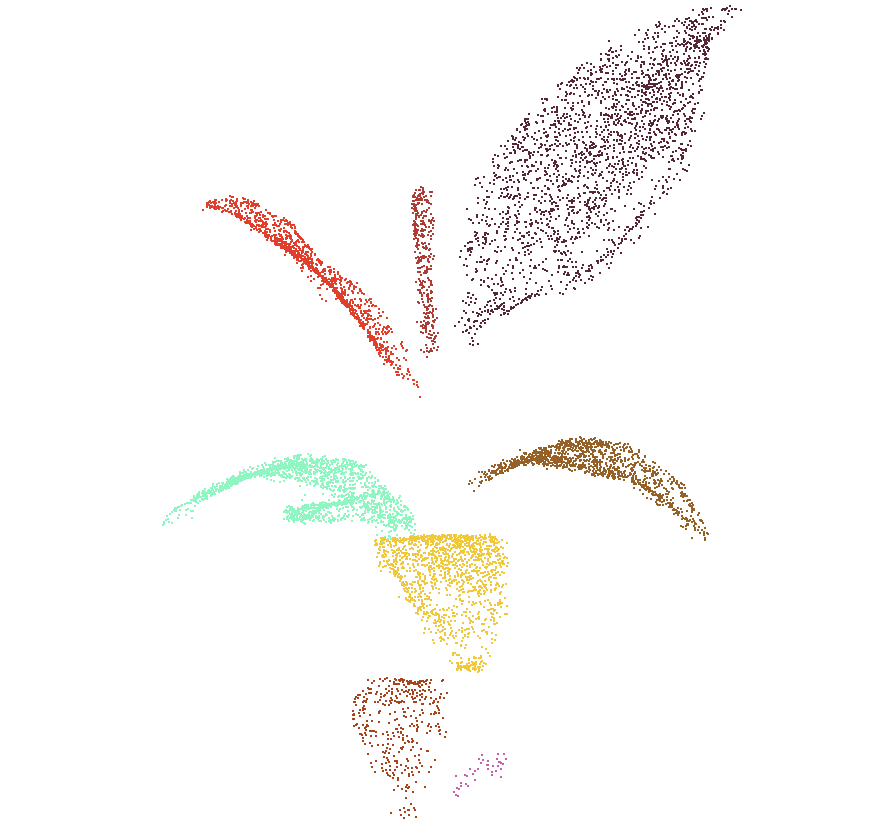
\includegraphics[height=4.5cm,width=4.5cm]{./Images/PipelineLeaveSegmentationStriped.png}
			\caption{Blatt-Segmentierung}
			\label{fig:PipelineLeaveSegmentation}
		\end{minipage}
	\end{figure}
}

\section{Quellen}
\begin{frame}[allowframebreaks]
    \frametitle{Referenzen}
    \bibliographystyle{ieeetr}
    \bibliography{./bibleografie.bib}
\end{frame}

\end{document}
